%!TEX root = Projektdokumentation_ClockPendulumAnalyzer.tex
\subsection{Sequenzdiagramm}
In diesem Kapitel werden einzelne Arbeitsabläufe anhand eines Sequenzdiagrammes dargestellt.
	\subsubsection{Start und Speichern einer Datenmessung}
    Dieses Sequenzdiagramm (Abbildung \ref{fig:sequence_save}) zeigt den Ablauf der Hauptfunktionalität.
    Zuerst werden alle zusätzlich benötigten Teilnehmer gestartet.
    Danach beginnt der Speichervorgang einzelner Datenmessungen.
    Dabei ruft das Programm die FIFO\footnote{First In, First Out}-Liste ab, welche durch die UART Kommunikation mit Messwerten befüllt wird.
    Sind 5 Datentupel aus der FIFO Liste gelesen, werden diese in der Datenbank gespeichert.
    \begin{figure}[H]
        \centering
        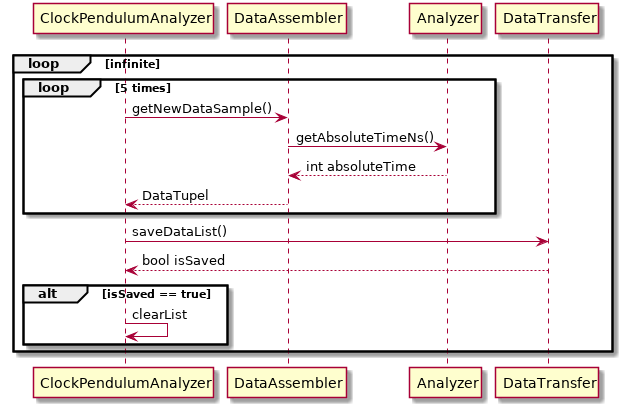
\includegraphics[width=\textwidth]{sequence_data_save.png}
        \caption{Sequenzdiagramm zum Speichern der Daten}
        \label{fig:sequence_save}
    \end{figure}

    \clearpage
    \subsubsection{Abrufen einer Datenmessung}
    Ein Webclient ruft als HTTP Request, über die definierte REST Schnittstelle Daten ab.
    Als Antwort erhält er eine JSON Struktur der Messdaten.
    Das ganze wird im Sequenzdiagramm (Abbildung \ref{fig:sequence_get}) unten abgebildet (mit dem Uhrennamen-Parameter als Beispiel).
    \begin{figure}[H]
        \centering
        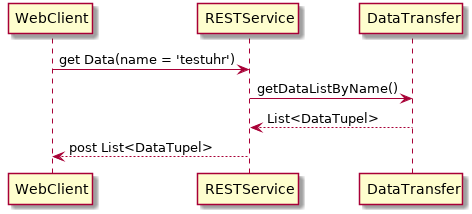
\includegraphics[width=.6\textwidth]{sequence_data_access.png}
        \caption{Sequenzdiagramm zum Aufrufen der Daten}
        \label{fig:sequence_get}
    \end{figure}
    %
	\subsubsection{Zählersystem}
	Die Software auf dem \hwb\ ist in C geschrieben und somit nicht objektorientiert. Dementsprechend sind die einzelnen Lebenslinien keine Objekte sondern eigene C-Dateien, deren Methoden entsprechend dem Diagramm aufgerufen werden. Die Akteure stellen dabei die Interrupt-Eingänge dar.
	\noindent Der Main-Loop, das eigentliche C-Programm, prüft alle 10 Millisekunden, ob ein Event gesetzt ist, oder ob noch Daten im USB-Kanal zum Senden vorhanden sind. Dementsprechend ist dieser Teil des Programmes nicht besonders zeitkritisch und kann problemlos zwischen den Interrupts verarbeitet werden.\\
	Die Interrupts des GPS-Moduls sind zeitkritisch und wie im Abschnitt \ref{cap:counter_realisation} beschrieben, von der höchsten Priorität. Darin werden die aktuellen Zählerwerte umgehend gespeichert und anschliessend der entsprechende Event gesetzt, welcher dann beim nächsten Durchgang des Main-Loops verarbeitet wird.
    Der gesamte Ablauf ist im Sequenzdiagramm in Abbildung \ref{fig:sequence_hwb} dargestellt.
 	\begin{figure}[H]
   		\centering
        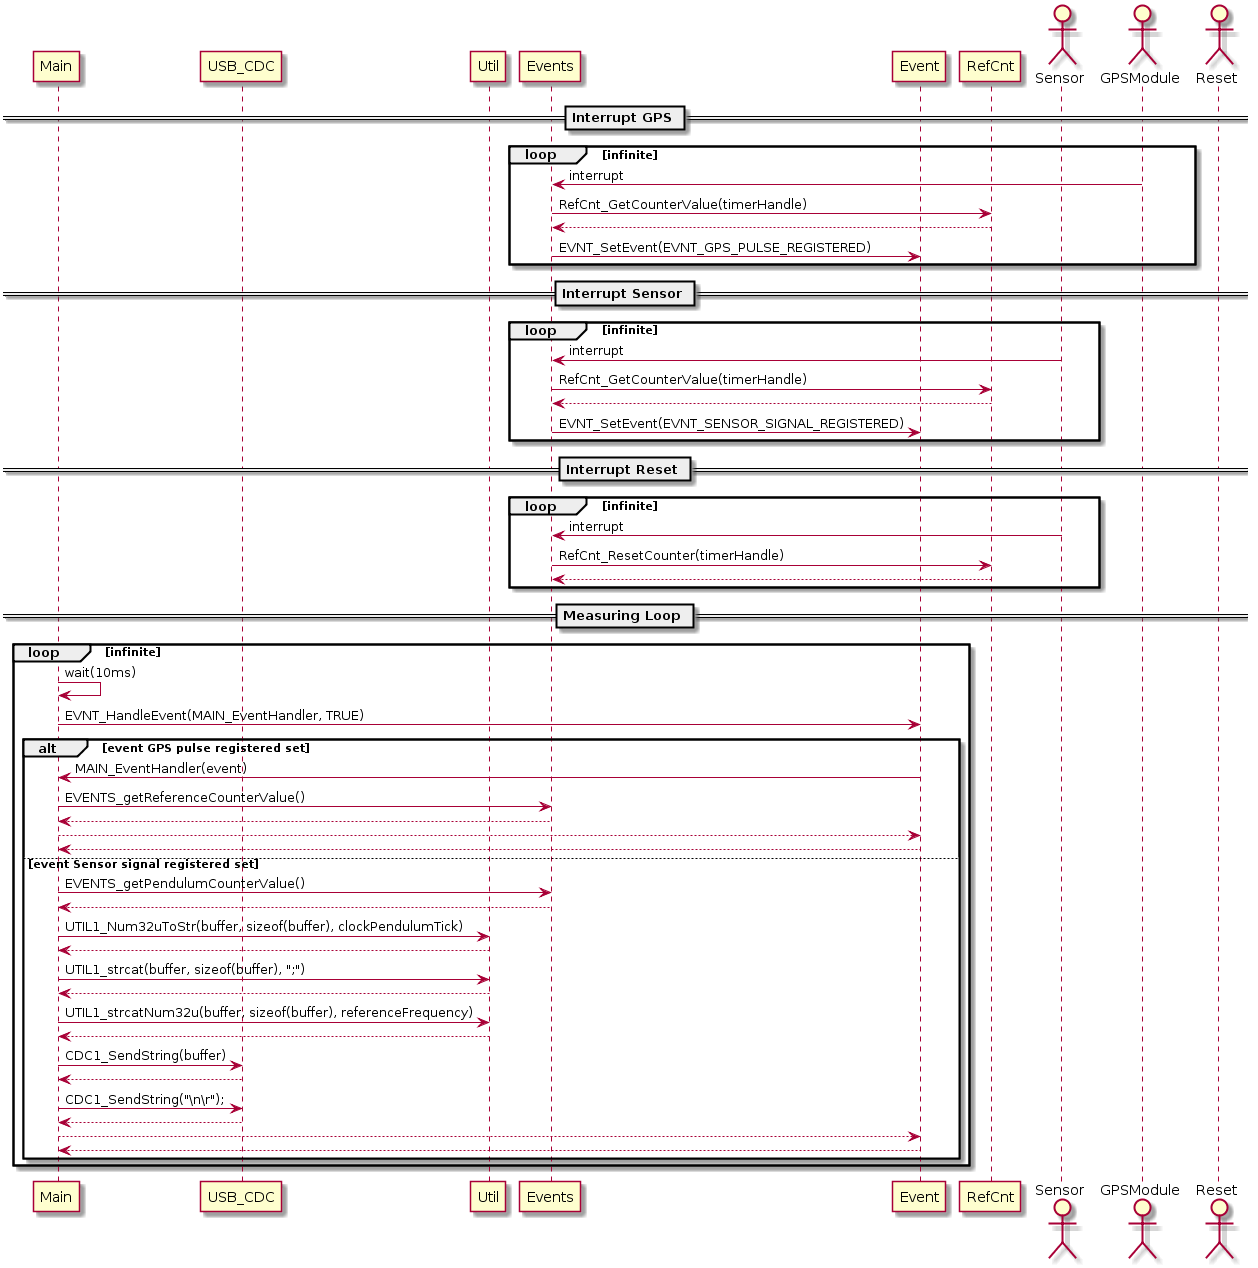
\includegraphics[width=\textwidth]{sequence_hwb.png}
        \caption{Sequenzdiagramm Zählersystem zur Pendelerfassung}
        \label{fig:sequence_hwb}
    \end{figure}